\chapter{GAN}
Ein \glqq Generative Adversarial Net\grqq{} besteht aus zwei Teilstücken. Der erste Teil wird \glqq generative model $G$\grqq{}
genannt und generiert auf Basis eines originalen Datensets neue Datensamples. Der zweite Teil nennt sich \glqq discriminative model $D$\grqq{}
und schätzt die Wahrscheinlichkeit, ob ein solches Sample, welches $G$ generiert, aus dem originalen Datenset stammt. $D$
selbst hat als Output also eine reele Zahl. \cite{8253599}
In den Worten der Autoren ausgedrückt ist ein \Gls{GAN} ein Spiel zwischen Geldfälschern und Polizisten:
\itenquote{The generative model can be thought of as analogous to a team of counterfeiters,
trying to produce fake currency and use it without detection, while the discriminative model is
analogous to the police, trying to detect the counterfeit currency. Competition in this game drives
both teams to improve their methods until the counterfeits are indistiguishable from the genuine
articles} \cite{8253599}.
Anders ausgedrückt versucht $G$ immer besser zu werden, um $D$ möglichst zu überlisten. $D$ hingegen sieht sich einem immer
besser werdenden $G$ gegenüber gestellt und muss seine eigenen Schwachstellen ausbessern, um $G$ entgegenzuhalten. Eine Architektur, die
so aufgebaut ist, dass sie sich gegenseitig immer weiter verbessert. Aus diesm Grund auch \glqq Generative \textbf{Adversarial} Net\grqq{} genannt.
\para
Im Endeffekt besteht das Ziel also darin, dass $D$ nicht mehr sagen kann, ob ein Sample von $G$ oder aus dem originalen Datenset stammt.
Somit sollte $D$ für alle Samples immer $\frac{1}{2}$ ausgeben. Dies bedeutet, dass ein Sample dieselbe Wahrscheinlichkeit
hat aus dem originalen Datenset oder aus dem generierten Set zu stammen und diese
beiden Datensets daher nicht mehr unterscheidbar sind.
Der Trainingsprozess für $G$ kann weiterhin als Maximierung der Fehlerwahrscheinlichkeit für $D$ angegeben werden. Dies entspricht also einem
Zwei-Spieler Minimax-Algorithmus, auf welchen in dieser Arbeit ebenfalls noch eingegangen wird.\cite{8253599}
\para
Das generative Modell $G$ sowie das unterscheidende Modell $D$ bestehen jeweils aus zwei \Glspl{Multilayer perceptron}. Dies hat
den Vorteil, dass die Modelle mittels \Gls{Backpropagation} trainiert werden können \cite{8253599}.

\section{Neuronale Netze - Multilayer Perceptron}
Da die Architektur des \Gls{GAN} auf zwei neuronalen Netzen beruht, wird in diesem Kapitel kurz darauf eingegangen. Dieser
Einschub gibt einen groben Überblick, hat aber nicht die Absicht, ein vertieftes Wissen zu vermitteln.
\para
Die neuronalen Netze sind, wie so manches, über die Zeit herangereift. Die Intention besteht nicht darin, das menschliche Gehirn
nachzubauen, sondern eher eine Art Modell für die Informationsverarbeitung zu beschreiben \cite{wiki:knn}. Wie in der Biologie versucht man dies
in diesen Netzen über Neuronen, wo auch der Name herrührt. Ein solches
Neuron bekommt als Eingabe eine Summe von gewichteten Werten, welche es durch eine sogenannte \glqq Aktivierungsfunktion\grqq{} in
einen Ausgabewert umwandelt.
\para
Am Anfang dieser Netzwerke stand das Perzeptron, welches nur ein
einziges künstliches Neuron beinhaltet und von Frank Rosenblatt beschrieben wurde.\cite{wiki:perzeptron} Danach hat man damit
begonnen, diese Neuronen über Layer miteinander zu verbinden, wobei man den ersten Layer als Input-Layer, die Layer dazwischen
als Hidden-Layer und den letzten Layer aus Output-Layer kennt. Der Output-Layer beinhaltet in einem einfachen \Gls{KNN} so viele
Neuronen, wie es Klassen gibt. Jedes dieser Output-Neuronen gibt die Wahrscheinlichkeit an, ob eine Eingabe zu der jeweiligen
Klasse gehört \cite{wiki:knn}.
\para
Ein solches neuronales Netz ist eigentlich eine Optimierungsaufgabe. In dem Fall geht es darum, am Ende eine Fehlerfunktion, welche
den Abstand des Ist- und Sollzustands beschreibt, zu minimieren. Je geringer der Fehler, desto besser klassifiziert das Netz. Die
Variablen, welche dabei angepasst werden können, sind die Gewichte, welche jeweils auf einer Verbindung zwischen zwei Neuronen liegen.
Wie wahrscheinlich jeder aufmerksame Leser erkennt, werden dies sehr schnell sehr viele Variablen, weswegen normale Verfahren wie
z.B. der Gradientenabstieg zwar eingesetzt werden können, aber sehr ineffizient sind.
Der Durchbruch dieser Netzwerke wurde daher erst mit der Beschreibung des \Gls{Backpropagation}-Algorithmus erzielt, welcher ein Spezialfall
des Gradientenabstiegverfahrens darstellt und die Gewichte aufgrund ihres Anteils am Fehler anpasst \cite{wiki:backpropagation}.
Heute gibt es sehr viele verschieden Arten und Architekturen von künstlichen neuronalen Netzen, auf welche nun nicht weiter eingegangen
wird.

\section{Funktionsweise}
Formell ausgedrückt besteht ein \Gls{GAN} aus zwei ableitbaren Funktionen $G(z;\theta_g)$ und $D(x,\theta_d)$, welche durch zwei \Glspl{Multilayer perceptron}
dargestellt werden. Dabei bilden jeweils $\theta_g$ sowie $\theta_d$ die Parameter der Netzwerke. Um die generierten Daten $p_g$ über ein Sample $x$ aus
dem originalen Datenset $p_{data}$ zu trainieren, wird eine Input-Noise-Funktion $p_z(z)$ definiert. $G(z;\theta_g)$ bildet dabei das
Mapping zwischen diesen Noise-Daten und dem originalen Datenset $p_{data}$.
Aus dem Noise wird also ein Sample erzeugt, welches möglichst mit den Samples aus $p_{data}$ korreliert.
$D(x)$ wiederum gibt einen einzelnen Skalar aus, der die Wahrscheinlichkeit beschreibt, ob ein Sample $x$ eher aus dem originalen Datenset $p_{data}$
als aus dem generierten Datenset $p_g$ (beinhaltet alle Samples von $G$) stammt.
$D$ wird nun so trainiert, um die Wahrscheinlichkeit zu maximieren, das korrekte Label einem Input-Sample $x$ zu geben. Dabei gibt es zwei Labels:
\glqq Stammt aus original Datenset\grqq{} und \glqq Stammt aus generiertem Datenset\grqq{}. Simultan dazu wird $G$ trainiert, um die Funktion
$\log(1 - D(G(z)))$ zu minimieren\cite[p.~1]{8253599}. In Worten: $G(z)$ generiert ein Sample aus den Noise-Daten.
Davon wird die Wahrscheinlichkeit berechnet, ob dieses Sample aus dem originalen Datenset stammt. Wird dieser Wert gross, das heisst,
$D$ hat das Gefühl, dass das generierte Sample aus dem originalen Datenset stammt, so geht der Wert innerhalb des Logarithmus gegen 0 und damit gegen $-\infty$.
Dadurch wird also über diese Minimierung erzielt, dass $G$ möglichst Daten generiert, die $D$ nicht dem generierten Datenset sondern dem originalen Datenset selbst zuweist.
Die Autoren verweisen hier auf die Tatsache, dass die beiden neuronalen Netze $D$ und $G$ ein
Zwei-Spieler minimax-Spiel mit der folgenden Value-Funktion $V(G,D)$ spielen \cite[p.~2]{8253599}:
\begin{align}
    \min_{G} \max_{D} V(D, G) = E_{x\sim p_{data}(x)}[\log D(x)] + E_{z\sim p_z(z)}[\log(1 - D(G(z)))]
\end{align}
Diese Value-Funktion definiert die Fehlerfunktion von $D$. Nachfolgend werden einige Gedanken des Autors dazu aufgeführt.\\
\textbf{Fall 1 - Discriminator macht alles richtig}:
\begin{align}
    D(x) = 1, D(G(z)) = 0 \Rightarrow \log(1) + \log(1 - 0) = \log(1) + \log(1) = 0
\end{align}
\textbf{Fall 2 - Discriminator weist $G(z)$ dem Datenset zu}:
\begin{align}
    D(x) = 1, D(G(z)) = 1 \Rightarrow \log(1) + \log(1 - 1) = \log(1) + \log(0) = -\infty
\end{align}
\textbf{Fall 3 - Discriminator kann nicht mehr unterscheiden}:\\
\begin{align}
    D(x) = \frac{1}{2}, D(G(z)) = \frac{1}{2} \Rightarrow \log(\frac{1}{2}) + \log(1 - \frac{1}{2}) = \log(\frac{1}{2}) + \log(\frac{1}{2}) = -\log(4) = -1.3862
\end{align}
Nach den Autoren bildet der Fall 3 das globale Minimum, welches eben nur erzielt werden kann, wenn der Discriminator nicht mehr zwischen
den beiden Datensets unterscheiden kann \cite[p.~4-5]{8253599}. Es gilt: $p_{data} = p_{g}$
\para
Nun stellt sich noch die Frage, wie denn genau $G$ lernt. Nach \glqq Computerphile\grqq{} erhält $G$ Informationen von $D$.
$G$ kennt also die Schwächen von $D$ und kann diese besser ausnützen. Dies geschieht über die Gradienten von $D$. \cite{youtube:gan}
\\TODO: Mapping besser von Noise z nach x darstellen
\newpage
\subsection{Einschub - Minimax}
Um zu verstehen, wieso es sich hierbei um einen solchen Minimax-Algorithmus handelt, wird in diesem Abschnitt ebendieser mit
Verweis auf die Gleichung 1 eingeführt. Der Algorithmus geht auf den Versuch zurück, für ein Zwei-Spieler-Spiel eine
schlaue KI zu erschaffen, die möglichst weit in die Zukunft sehen und abschätzen kann, was der Gegener tun wird.
Dabei geht man davon aus, dass der Gegner immer so agiert, damit er seine Gewinnwahrscheinlichkeit maximiert und die
der KI minimiert.\cite{towardsdatascience:minimax} Die Züge, welche gemacht werden können, werden über einen sogenannten
Game-Tree dargestellt. In Abbildung 2.1 ist der Game-Tree für ein \Gls{GAN} gegeben. Jeder Layer stellt einen Zug in diesem
\begin{figure}[h!]
    \begin{center}
        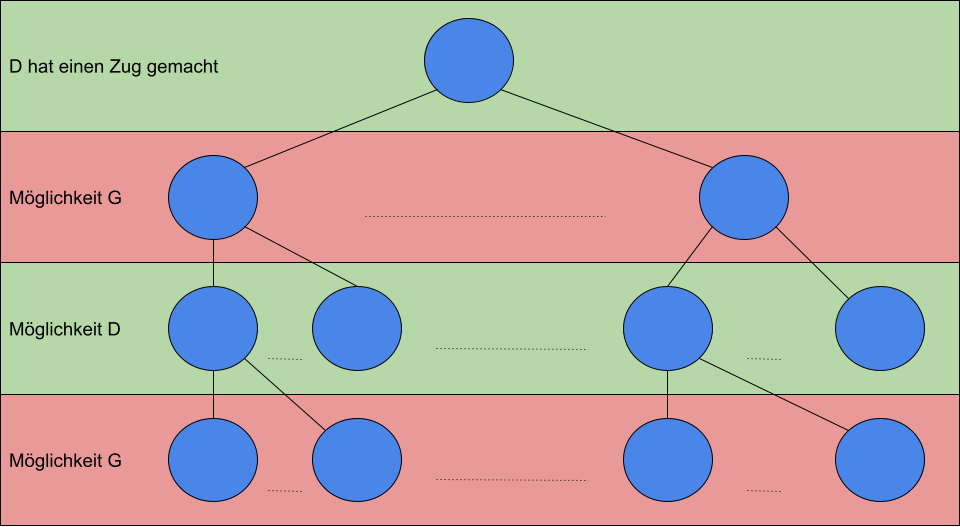
\includegraphics[width=0.5\textwidth]{../common/02_main/resources/03_gan_game_tree.png}
    \end{center}
    \caption{Leerer GAN-Game-Tree}
    \label{fig:Leerer GAN-Game-Tree}
\end{figure}
Spiel dar. Innerhalb eines Zuges gibt es viele Möglichkeiten. Jede dieser Möglichkeiten wird über einen Node dargestellt.
Für ein \Gls{GAN} sind dies alle möglichen Zustände der Variablen, des neuronalen Netzwerks. Der Branching-Faktor ist also
sehr gross. In der Gleichung 1 geht es um die Maximierung für $D$, weswegen die grünen Layer zu $D$ gehören. In diesen Zügen
soll der Algorithmus die Value-Funktion $V(G,D)$ für einen Node aus seinen Nachfolgern maximal wählen. Hingegen soll $G$ minimiert werden, weswegen
die roten Layer zu $G$ gehören. Innerhalb dieser Layer wird der minimale Wert der nachfolge States bevorzugt. Ist eine gewisse
Tiefe erreicht worden, oder es gibt keine Nachfolge-States mehr, dann wird die Value-Funktion $V(G,D)$ für diese States aufgerufen und für den
jeweiligen Status der Wert berechnet. Abbildung 2.2 zeigt einen möglichen ausgefüllten Game-Tree über drei Stufen hinweg.
\begin{figure}[h!]
    \begin{center}
        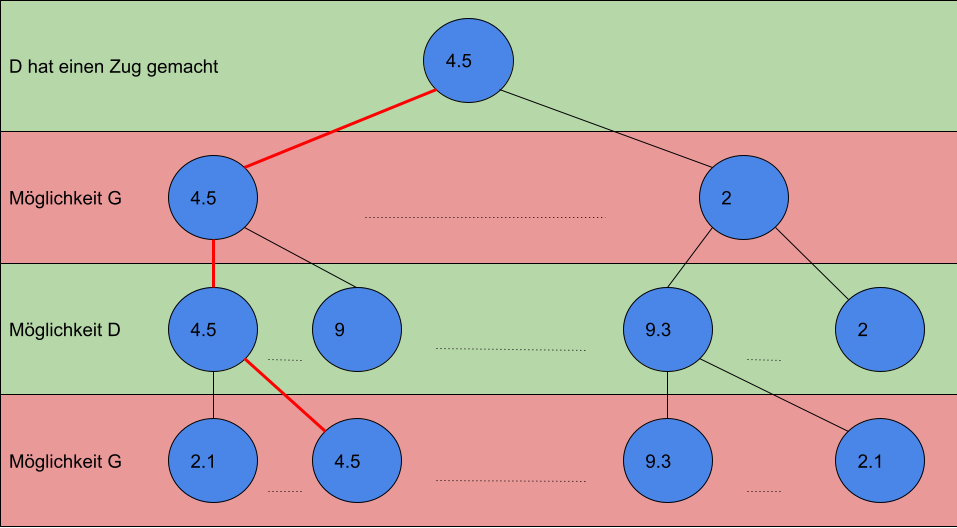
\includegraphics[width=0.5\textwidth]{../common/02_main/resources/04_gan_game_tree_filled.png}
    \end{center}
    \caption{Berechneter GAN-Game-Tree}
    \label{fig:Berechneter GAN-Game-Tree}
\end{figure}
Der rote Pfad bildet nach aktuellem Kentnisstand der beste Weg für $D$, und wird diesen wählen unter der Annahme,
dass $G$ wiederum den Weg wählen wird, welcher für $G$ am besten ist.
\section{Resultate}
Beschreibe einige Ergebnisse auch aus dem Abstract.
\section{Im Vergleich - Vor- und Nachteile}
Weitere möglichkeiten, Samples aus Daten zu generieren aufzeigen und evtl. Vergleich zu GAN.